\newpage


\section{Przegląd metod detekcji web scrapingu}\label{sec:przeglad-rozwiazan}

\subsection{Rate Limiting}\label{subsec:rate-limiting}

Rate Limiting to technika kontrolująca tempo, w jakim klienci mogą wysyłać żądania do serwera API\@.
W tym celu zlicza się liczbę żądań w określonym przedziale czasowym, a następnie ustala, czy ich częstotliwość nie przekracza maksymalnego dopuszczalnego progu~\cite{api-rate-limit-adoption}.

Rozwiązanie zazwyczaj polega na kalkulacji czasu między każdym żądaniem z każdego adresu IP\@.
W przypadku, kiedy liczba żądań z danego adresu IP przekroczy ustalony limit w danym oknie czasowym, żądanie kończy się odpowiednim błędem.
W tym przypadku adres IP służy jako identyfikator klienta~\cite{cloudflare-what-is-rate-limiting}.
Nie jest to jednak jedyne rozwiązanie, jako że dopuszcza się również identyfikatory innego rodzaju.

Brak rate limitingu API jest, według \emph{OWASP API Security Top 10}, uznawany za podatność.
W punkcie \emph{API4:2019 Lack of Resources \& Rate Limiting}, autorzy wskazują, że:\@
\begin{displayquote}[\citetitle*{owasp-api-security-top-10}~\cite{owasp-api-security-top-10}, tłum. własne]
    ``Żądania API zużywają zasoby takie jak sieć, CPU, pamięć i miejsce na dysku.
    Ilość zasobów potrzebnych do zaspokojenia żądania w dużej mierze zależy od danych wejściowych użytkownika i logiki biznesowej koncówki.
    Należy również wziąć pod uwagę fakt, że żądania od wielu klientów API konkurują o te same zasoby.
    API jest podatne na problemy, jeśli brakuje przynajmniej jednego z następujących limitów lub są one ustawione nieodpowiednio (np.\ zbyt niskie/wysokie):
    \begin{itemize}
        \item limit czasu wykonania,
        \item maksymalna alokowana pamięć,
        \item liczba deskryptorów plików,
        \item liczba procesów,
        \item rozmiar ładunku żądania (np.\ przesyłane pliki),
        \item liczba żądań na klienta/zasób,
        \item liczba rekordów na stronę zwracanych w pojedynczej odpowiedzi na żądanie.''
    \end{itemize}
\end{displayquote}

Rate Limiting stosuje się do ochrony ograniczonych zasobów, obrony przed atakami typu odmowa dostępu (ang. \emph{DoS, Denial of Service})
oraz blokowania aktywności botów generujących duże nadużycia.
Scrapery, będąc automatycznym oprogramowaniem, często kreują dużą liczbę zapytań w krótkim czasie, znacznie większą niż człowiek podczas standardowego korzystania z serwisu.
Istotne jest zatem takie skonfigurowanie reguł rate limitingu, aby znaleźć swoisty złoty środek, pozwalający na zablokowanie zautomatyzowanego pobierania danych bez jednoczesnego ograniczania dostępu prawdziwym użytkownikom.

\newpage

\subsection{Reverse Proxy --- blokowanie oparte na regułach}\label{subsec:reverse-proxy}

Termin proxy, w dziedzinie sieci komputerowych, określa aplikacje serwerową, która działa jako pośrednik między klientem wysyłającym żądanie a serwerem docelowym.
Wyróżnia się dwa główne typy proxy: forward proxy i reverse proxy.
Oba z nich działają na brzegu sieci.
W uproszczeniu, pierwszy z nich pośredniczy między klientem a internetem, podczas gdy drugi zarządza ruchem przychodzącym z internetu do serwerów.
Uszczegóławiając, reverse proxy najczęściej znajduje się na brzegu sieci przed jednym lub wieloma serwerami.
Klient wysyła żądanie do serwera proxy, a ten je przechwytuje i przekazuje do serwerów docelowych~\cite{cloudflare-what-is-reverse-proxy}.
Działanie reverse proxy zostało przedstawione na \autoref{fig:reverse-proxy}.

\begin{figure}[H]
    \centering
    \captionsetup{width=.7\linewidth}
    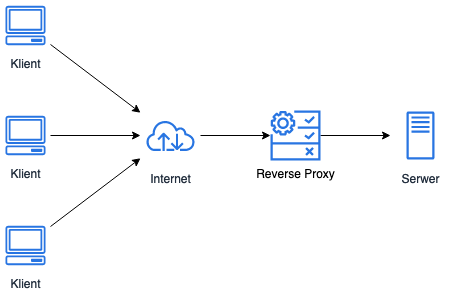
\includegraphics[width=0.8\textwidth]{img/reverse-proxy}
    \caption{Uproszczony schemat działania reverse proxy}
    \label{fig:reverse-proxy}
\end{figure}

Serwery reverse proxy znajdują swoje zastosowanie w detekcji web scrapingu ze względu na swoją zdolność do filtrowania ruchu przychodzącego.
Jak wskazano w \autoref{subsec:scraper}, ruch sieciowy generowany przez scrapery odznacza się niejednokrotnie charakterystycznymi cechami.
Na podstawie każdego z punktów w wspomnianym \autoref{subsec:scraper} można stworzyć regułę blokującą web scraping.

\newpage

\subsection{Browser Fingerprinting}\label{subsec:browser-fingerprinting}

Browser Fingerprint --- odcisk przeglądarki --- to zestaw informacji związanych z środowiskiem przeglądarki internetowej użytkownika, od fizycznego sprzętu, poprzez system operacyjny, aż do oprogramowania i jego konfiguracji~\cite{browser-fingerprinting-a-survey}.
Browser Fingerprinting to proces zbierania i analizy informacji tworzących odcisk przeglądarki.
Proces ten wykorzystuje się w celu identyfikacji i śledzenia użytkowników.
Dąż się do zgromadzenia możliwie wielu rekordów, które połączone razem tworzą unikalną kombinację jednoznacznie identyfikującą użytkownika~\cite{fingerprint-browser-fingerprinting}.
Informacje te najczęściej pochodzą z nagłówków HTTP oraz skryptów uruchamianych bezpośrednio w kontekście przeglądarki internetowej użytkownika.
Zebrane informacje mogą zawierać m.in.:
\begin{itemize}
    \item specyfikacje sprzętową: wersja urządzenia, rozdzielczość ekranu, poziom baterii, pamięć urządzenia, informacje nt. procesora (CPU) i karty graficznej (GPU),
    \item informacje o systemie operacyjnym i przeglądarce: typ i wersja systemu operacyjnego, typ i wersja przeglądarki internetowej, wtyczki zainstalowane w przeglądarce internetowej, obecność blokera reklam, wykorzystywany układ klawiatury, ustawienia przeglądarki (preferowany język, opcje śledzenia, wspieranie ciasteczek), ustawienia systemowe (strefa czasowa, zainstalowane czcionki), parametry WebGL (Web Graphics Library)
    \item informacje sieciowe: adres IP, szczegóły sesji TSL~\cite{browser-fingerprinting-a-survey,zitadel-browser-fingerprinting,zenrows-browser-fingerprinting,fingerprint-browser-fingerprinting}.
\end{itemize}
\noindent Przykładowy odcisk przeglądarki został przedstawiony w \autoref{tab:http-js-attributes}.

Browser Fingerprinting znajduje zastosowanie jako metoda detekcji web scrapingu.
Poprzez zbieranie odcisku przeglądarki i tworzeniu dla niego identyfikatora, możemy wymagać jego podania, tym samym blokując API web scraping.
Istnieją określone elementy odcisku sugerujące użycie metod automatyzacji~\cite{zenrows-browser-fingerprinting}.
Przykładowo, przeglądarki uruchomione przez biblioteki opisywane w \autoref{subsubsec:browser-scraping-theory} charakteryzują się:
ekranem o rozdzielczości 0x0 (Headless Browser),
WebGL z dostawcą \texttt{Brian Paul} lub \texttt{Mesa OffScreen} (Headless Chrome),
User-Agentem zawierającym \texttt{"PhantomJS"}, \texttt{"Headless"}, \texttt{"Electron"} lub \texttt{"slimerjs"},
brakiem zainstalowanych wtyczek, brakiem wspieranych kodeków wideo itd.
Ponadto, scrapery często są uruchomione w chmurach obliczeniowych bez urządzeń peryferyjnych lub środowiska graficznego.

\begin{table}[p]
    \small
    \centering
    \begin{tabular}{|p{0.35\linewidth} | p{0.6\linewidth}|}
        \hline
        \textbf{Atrybut}             & \textbf{Wartość}                                                                                                                                                                                                                                                                                                                                                                                                                              \\ \hline
        User Agent                   & Mozilla/5.0 (Macintosh; Intel Mac OS X 10.15; rv:122.0) Gecko/20100101 Firefox/122.0                                                                                                                                                                                                                                                                                                                                                          \\ \hline
        Platforma                    & MacIntel                                                                                                                                                                                                                                                                                                                                                                                                                                      \\ \hline
        Strefa czasowa               & UTC+01:00 (-60)                                                                                                                                                                                                                                                                                                                                                                                                                               \\ \hline
        Język                        & en-US,en,pl                                                                                                                                                                                                                                                                                                                                                                                                                                   \\ \hline
        Szczegóły ekranu             & szerokość: 1680, wysokość: 1050, depth: 24, dostępna wysokość: 1050, dostępna szerokość: 1680 i inne                                                                                                                                                                                                                                                                                                                                          \\ \hline
        Canvas                       & 
\includegraphics[width=0.9\linewidth]{img/fingerprint-cavas}                                                                                                                                                                                                                                                                                                                                                                                  \\ \hline
        Dostawca WebGL               & Apple                                                                                                                                                                                                                                                                                                                                                                                                                                         \\ \hline
        Renderujący WebGL            & Apple M1                                                                                                                                                                                                                                                                                                                                                                                                                                      \\ \hline
        Dane WebGL                   & 
\includegraphics[width=0.6\linewidth]{img/fingerprint-webgl}                                                                                                                                                                                                                                                                                                                                                                                  \\ \hline
        Parametry WebGL              & Wykryto 26 różnych rozszerzeń.\ Przeanalizowano 25 różnych parametrów ogólnych i 36 różnych precyzji shaderów.                                                                                                                                                                                                                                                                                                                                \\ \hline
        Lista fontów (JS)            & Al Bayan, Al Nile, Al Tarikh, American Typewriter, Andale Mono i 181 innych                                                                                                                                                                                                                                                                                                                                                                   \\ \hline
        Wtyczki &
        --- PDF Viewer; Portable Document Format; internal-pdf-viewer\newline
        --- Chrome PDF Viewer; Portable Document Format; internal-pdf-viewer.\newline
        oraz 3 inne \\ \hline
        Wykorzystanie AdBlock        & Tak                                                                                                                                                                                                                                                                                                                                                                                                                                           \\ \hline
        Do Not Track                 & Tak                                                                                                                                                                                                                                                                                                                                                                                                                                           \\ \hline
        Atrybuty Navigator           & Wykryto 45 obiektów                                                                                                                                                                                                                                                                                                                                                                                                                           \\ \hline
        Urządzenia multimedialne     & 2 wejścia audio, 1 wejście video                                                                                                                                                                                                                                                                                                                                                                                                              \\ \hline
        Kontekst audio               & częstotliwość próbkowania: 48000, stan: wstrzymano                                                                                                                                                                                                                                                                                                                                                                                            \\ \hline
        Wspierane rozszerzenia audio & audio/aac : możliwe, audio/flac : możliwe, audio/mpeg : możliwe, audio/ogg; codecs=\("\)flac\("\)  : prawdopodobnie, audio/ogg; codecs=\("\)vorbis\("\) : prawdopodobnie, audio/ogg; codecs=\("\)opus\("\) : prawdopodobnie, audio/wav; codecs=\("\)1\("\) : prawdopodobnie, audio/webm; codecs=\("\)vorbis\("\) : prawdopodobnie, audio/webm; codecs=\("\)opus\("\) : prawdopodobnie, audio/mp4; codecs=\("\)mp4a\_40\_2\("\) : prawdopodobnie \\ \hline
        Wspierane rozszerzenia video & video/mp4; codecs=\("\)flac\("\) : prawdopodobnie, video/ogg; codecs=\("\)theora\("\) : prawdopodobnie, video/ogg; codecs=\("\)opus\("\) : prawdopodobnie, video/webm; codecs=\("\)vp9, opus\("\) : prawdopodobnie, video/webm; codecs=\("\)vp8, vorbis\("\) : prawdopodobnie,                                                                                                                                                                \\ \hline
        Dostępne elementy            & Location Bar, Menu Bar, Personal Bar, Status Bar, Tool Bar, Local Storage, Session Storage, IndexedDB, Ciasteczka                                                                                                                                                                                                                                                                                                                             \\ \hline
    \end{tabular}
    \caption{Wybrane atrybuty odcisku przeglądarki autora pracy\\Tabela powstała przy pomocy serwisu AM I UNIQUE?\\(\url{https://amiunique.org/})}
    \label{tab:http-js-attributes}
\end{table}

%\begin{enumerate}
%    \item specyfikacje sprzętową:
%    \begin{itemize}
%        \item wersja urządzenia,
%        \item rozdzielczość ekranu,
%        \item poziom baterii,
%        \item pamięć urządzenia,
%        \item informacje nt. procesora (CPU),
%        \item informacje nt. karty graficznej (GPU),
%    \end{itemize}
%    \item informacje o systemie operacyjnym i przeglądarce:
%    \begin{itemize}
%        \item typ i wersja systemu operacyjnego,
%        \item typ i wersja przeglądarki internetowej,
%        \item wtyczki zainstalowane w przeglądarce internetowej (w tym obecność blokera reklam),
%        \item wykorzystywany układ klawiatury,
%        \item ustawienia przeglądarki (preferowany język, opcje śledzenia, wspieranie ciasteczek),
%        \item ustawienia systemowe (strefa czasowa, zainstalowane czcionki),
%        \item parametry WebGL (Web Graphics Library)
%    \end{itemize}
%    \item informacje sieciowe:
%    \begin{itemize}
%        \item adres IP,
%        \item szczegóły sesji TSL~\cite{browser-fingerprinting-a-survey,zitadel-browser-fingerprinting,zenrows-browser-fingerprinting,fingerprint-browser-fingerprinting}.
%    \end{itemize}
%\end{enumerate}
